\documentclass[]{homework}
\usepackage{multirow}
\usepackage{graphicx}
\usepackage{tikz}
\usetikzlibrary{arrows,automata}

\begin{document}
\header{CS5340}{Project Proposal}{Shawn Tan \& Davin Choo}

This is super duper uber draft, I basically just copied shit from my interim report into this.
\section{Introduction}
With the advent of Web 2.0, sites with forums, or similar thread-based discussion features are increasingly common.
In this project,our goal is to predict updates in such threads.

Many of the popular Web 2.0 sites have comment features. This suggests that content on the web is increasingly being created by users alongside content providers. While mining structured, curated content from sites like Amazon, for data like prices is easy and effective, data that can be obtained from user-generated content are of a different nature. One may be able to infer public sentiment about a given product that would not be readily available from an e-commerce site.
%we are predicting web 2.0 updates
In some cases, news may travel more quickly through such online community discussion than through traditional media. Users also typicaly discuss purchased products bought online via these forums, and companies that want to get timely feedback about their product should turn to data mined from such sites.

A naive way of getting timely updates is to aggressively hit the pages repeatedly downloading the pages at a very frequent rate. However, the number of pages in a forum site are far too large to perform this efficiently on every forum. One way to minimise this cost would be to look at the time differences between previous posts to estimate the arrival of the next one. We believe that the content of the thread has information that can give a better estimate of the time interval between the last post and a new one.


For example, a thread in a technical forum about a Linux distribution may start out as a question. Subsequent questions that attempt to either clarify or expand on the original question may then be posted, resulting in a quick flurry of messages. Eventually, a more technically savvy user of the forum may come up with a solution, and the thread may eventually slow down after a series of messages thanking the problem solver. Suppose 10 days later, someone with a slight variation of the same problem posts on the thread again. A crawler that estimate's update rates solely on the age of the thread to determine its download rate of the thread may not update itself with the thread.
%TODO:Bring to beginning and shorten to 1 or 2 sentences after the problem statement.
%as rate increase, timeliness become more important
% talk about consequences of naive method

Let us define all such thread-based discussion styled sites as forums. Ideally, an incremental crawler of such user-generated content should be able to maintain a fresh and complete database of content of the forum that it is monitoring. However, doing so with the previously mentioned naive method would (1) incur excessive costs when downloading un-updated pages, and (2) raise the possibility of the web master blocking the requester's IP address.

%Thus, we need a strategy of revisiting pages that will reduce the cost of downloading unchanged pages, while at the same time downloading them as soon as possible after it's update. 
This year-long project proposes to use content-based features of a given thread to predict its next update time. We argue, that the content within the posts of the thread should be important in predicting the thread updates, and propose our approach to solving the problem.


\section{Proposed Method}

From our initial analysis of the extracted data from the Hardwarezone forums, we have made the following observations about non-sticky threads in the forum:
\begin{enumerate}
	\item There are threads that are very short-lived, and some that are long lived. This is largely dependent on the thread content. For example, a user looking to buy/sell a product that no one has an interest in. %TODO cite paper that shows the lifetime of threads
	\item The long-lived threads typically have a pattern to the frequency of postings. A high frequency of posts are seen around lunch time (12-3 PM) and another spike is seen during the night at 9 PM. (Figure \ref{sleepcycle}). It is yet to be determined if this type of cycle is site-wide or thread-specific.
\end{enumerate}
Our initial model aims to incorporate these observations. A new thread (represented by $q_0$ which only has one post, may transition to either an active or active but `sleeping' thread, or an inactive thread.
%This is to account for the fact that a thread may be active, but the thread has a lack of activity, due to the fact that its' users are sleeping or working.


\begin{figure}
	\begin{center}
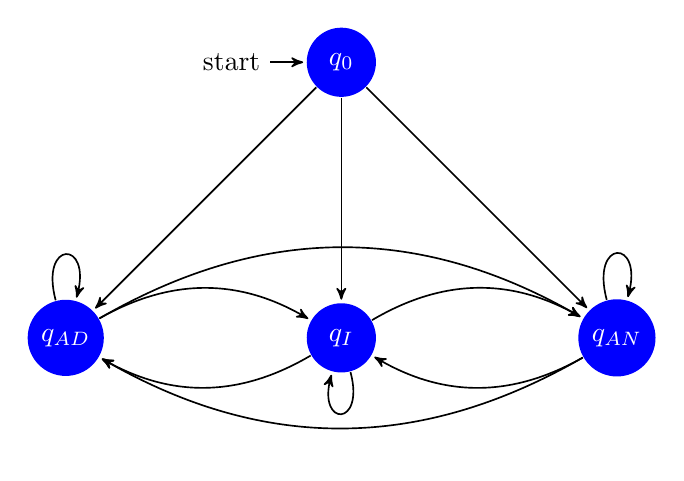
\begin{tikzpicture}[->,>=stealth',shorten >=1pt,auto,node distance=3.5cm,
                    semithick]
  \tikzstyle{every state}=[fill=blue,draw=none,text=white]

  \node[initial,state] (q0)                    {$q_0$};
  \node[state]         (IN) [below of=q0] {$q_I$};
  \node[state]         (AD) [left of=IN] {$q_{AD}$};
  \node[state]         (AN) [right of=IN] {$q_{AN}$};

  \path (q0) edge              node {} (AD)
 			 edge 			   node {} (AN)
			 edge 			   node {} (IN)
		(AD) edge [loop above] node {}(AD)
			 edge [bend left]  node {}(AN)
			 edge [bend left]  node {}(IN)
		(AN) edge [bend left]  node {}(AD)
			 edge [loop above] node {}(AN)
			 edge [bend left]  node {}(IN)
		(IN) edge [bend left]  node {}(AD)
			 edge [bend left]  node {}(AN)
			 edge [loop below] node {}(IN);
\end{tikzpicture}

\end{center}
	\caption{Preliminary modelling of a thread as a probabilistic automaton}\label{spaceship}
\end{figure}
We define active here as threads with a high post frequency, and inactive threads and as posts with low post frequency. Since our observations show that threads have different levels of post frequencies due to usage patterns consistent with user's sleep cycles and work commitment, we use 3 states in total to represent the state of a thread with more than 2 posts. A `day' state (represented by $q_{AD}$) and a `night' state (represented by $q_{ND}$). The inactive threads are represented by the state $q_I$
%Our initial model aims to incorporate these observations. A new thread (represented by $q_0$) which only has one post, may transition into either an active or inactive state (represented by $q_A$ respectively). We define active here as threads with high post frequency, and inactive threads as posts with low post frequency. Since our observations show that threads have different levels of post frequencies due to usage patterns consistent with user's sleep cycles, we use four states in total to represent the state of a thread with more than 2 posts, a `day' state and a `night' state (represented by $q_D,q_N$). These four states form a clique. Each of these states produce a set of observations that we can use to identify the state that a thread is in.

The intuition behind this is the fact that active threads can transition to an inactive state, but the presence of a new post is able to spark off a new discussion within the thread, causing it to be an active thread again.

The graphical representation of this automata is seen in Figure \ref{spaceship}.


Our initial collection of data to identify changes in state for active threads to inactive threads do not show any observable patterns. More data has to be collected and analysed before conclusions can be made. Statistics of textual content, along with data for a more complete set of threads may provide some insight to their behaviour.


\section{Proposed Plan}
\end{document}
